\documentclass[9pt]{entcs} 
%\documentstyle{elsart}
\usepackage{entcsmacro}

\usepackage{lscape}
%\usepackage[T1]{fontenc}
%\usepackage[utf8]{inputenc} %latin1
\usepackage{amsmath,amssymb}
\usepackage{xparse}
\usepackage{url}
\usepackage{graphicx}
\usepackage[caption=false]{subfig}
\usepackage{braket}
\usepackage{amsfonts}

\let\proof\relax %esses comando e o de baixo evitam conflito do ambiente proof de amsthm com outros pacotes
\let\endproof\relax
\usepackage{amsthm}

\usepackage{fancyhdr}
\usepackage{comment}
\usepackage{float}
\usepackage{mathtools}
\usepackage{xspace}
\usepackage[inline]{enumitem}
\usepackage[export]{adjustbox}
\usepackage[numbers]{natbib}
\usepackage{marginnote}
\usepackage[usenames, dvipsnames]{color}
\usepackage[nameinlink, nosort]{cleveref}
%\usepackage{multirow}
% \usepackage{slashbox}
\usepackage{diagbox}
%\usepackage{slashbox}
\sloppy
%\usepackage{mathtools}
\usepackage{ tipa } %para angulos/dobras
\DeclarePairedDelimiter{\ceil}{\lceil}{\rceil}

\newtheorem{teo}{Theorem}[section]
\newtheorem{lema}{Lemma}[section]
\newtheorem{defi}{Definition}[section]
\newtheorem{coro}{Corollary}[section]
%\newtheorem{pro}{Proposition}[section]
%\newtheorem{fac}{Fact}[section]
%\newtheorem{prove}{pf}[section]
%\renewcommand{\proofname}{pf}[section]
%%%


\newcommand{\Nat}{{\mathbb N}}
\newcommand{\Real}{{\mathbb R}}
\def\lastname{author1, author2, author3, author4, author5}
\begin{document}
\begin{frontmatter}
  \title{Relationship Between VPT, EPT and $B_1$-EPG Graphs}
  


\begin{abstract}
This paper presents how main result the prove that every Chordal $B_1$-EPG graph is also a VPT and EPT graph. In addition, we show that while $B_1$-EPG-Helly graphs recognition is a $\textsc{NP}$-complete problem, there are subclasses itself contained in $B_1$-EPG-Helly for which the recognition is polynomial, e.g. Block graphs. In particular we present characterizations for Cographs, Bipartite, Block, Cactus and Line-graph of Bipartite  graphs. % that are new results beyond those already known in the literature.
\end{abstract}

\begin{keyword}
%% keywords here, in the form: keyword \sep keyword
Edge-intersection of paths on a grid \sep Edge-intersection graph of paths in a tree  \sep Helly property \sep Intersection graphs \sep Single bend paths \sep Vertex-intersection graph of paths in a tree.
\end{keyword}

\end{frontmatter}

% \linenumbers

\section{Introduction}

The searches on path intersection graph are approached considering intersections from vertices or edges. Cases where models of intersection have a tree as host appear first in the literature e.g. \cite{gavril1974intersection, golumbic1985edge, golumbic1985}, later representations on a grid were considered, e.g. \cite{golumbic2009,golumbic2013, golumbic2013intersection}. More details on each intersection model will be given in the following text.

The research of paths whose host is a tree starts in 1974 with Gavril~\cite{gavril1974intersection} who proved that a graph $G$ is an intersection graph of subtrees family of a tree if and only if $G$ is a chordal graph. An undirected graph $G$ is called an EPT graph if it is the edge intersection graph of a family of paths in a tree. Let $P$ be a family of paths on a host tree $T$ . Two types of intersection graphs from the pair $<P,T>$ are defined, namely VPT and EPT graphs.
The \textit{edge intersection graph} of $P$, EPT(P), has vertices which correspond to the members of P, and two vertices are adjacent in EPT(P) if and only if the corresponding paths in P share at least one edge in T. Similarly, the \textit{vertex intersection graph} of P, VPT(P), has vertices which correspond to the members of P, and two vertices are adjacent in VPT(P) if and only if the corresponding paths in P share at least one vertex in T.

VPT and EPT graphs are incomparable families of graphs. However, when the maximum degree of the host tree is restricted to 3 the family of
VPT graphs coincides with the family of EPT graphs, \cite{alcon2010necessary}.

 Golumbic, Lipshteyn and Stern defined in 2009 the class of EPG graphs, as the  intersection graph of edge paths on a grid. An EPG graph $G$ is a graph that admits a representation where its vertices correspond to paths in a grid $Q$, such that two vertices of $G$ are adjacent if and only if their corresponding paths in $Q$ have a common edge. If the paths in the representation have at most $k$ changes of direction  (bends), we say that it is a  $B_k$-EPG representation. In particular when the paths of this representation have at most 1 bend we say that this is a $B_1$-EPG representation or single bend representation for EPG graphs.  A collection $C$ of sets satisfies the Helly property when every sub-collection of $C$ that is pairwise intersecting has at least one common element. 


\begin{defi} \label{defi:tortasFrame}

Let $ Q $ be a grid and let $ (a_1, b),$ $(a_2, b),$ $(a_3, b),$ $(a_4, b)$ be a 4-star as depicted in Figure~\ref{fig:piesInGrid}(a). Let $ \mathcal{P} = \{P_1, \dots , P_4\}$ be a collection of paths each containing exactly two edges of the $4$-star:

\begin{itemize}
\item A \emph{true pie} is a representation where each $P_i$ of $ \mathcal{P} $ forms a bend in $b$.

\item A \emph {false pie} is a representation where two of the paths $P_i$ do not contain bends, while the remaining two do not share an edge. 

%In false pie only 2 paths not adjacent do bend in $b$.
%\vspace{-0.5cm}
%\input{recorteGrade.tex}
\begin{figure}[htb]
  \centering
%segundo bloco de figuras
  \begin{tabular}{c c c c c }
    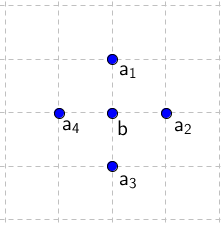
\includegraphics[width=3.5cm]{img/disposicaoTortaGrid3}    
    & &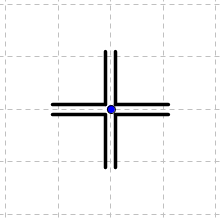
\includegraphics[width=3.5cm]{img/truePieGrid} 
    & &
 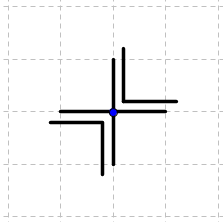
\includegraphics[width=3.5cm]{img/falsePieGrid} \\%[\abovecaptionskip]
    {\footnotesize (a) 4-star in grid.}  & &  {\footnotesize (b) True pie.} & & {\footnotesize (c) False pie.} %\label{fig:frame}
  \end{tabular}
  \caption{$B_{1}$-EPG representation of the induced cycle of size 4 as pies with emphasis in center $b$.}\label{fig:piesInGrid}
\end{figure} 

%\vspace{-0.5cm}
\end{itemize}
\end{defi}


A \textit{diamond} is a graph with vertex set $\{a, b, c, d\}$ and edge set $\{ab, ac,bc, bd,cd\}$, see Figure~\ref{fig:diamond}. A graph is diamond-free if it does not contain a diamond as induced subgraph.

 \begin{figure}[htb]	
 \center%6.3
 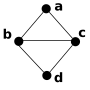
\includegraphics[width=2.2cm]{./img/diamond.png}
 \caption{Diamond graph.}
\label{fig:diamond}
\end{figure}  
 


In an EPG representation of a graph $G$, a clique $C$  is an \textit{edge-clique} if all the paths that correspond to the vertices of $C$ share a common edge of the grid $Q$, see Figure~\ref{fig:cliquesRepresentation}(a). %A \textit{claw} in a grid consists of three grid edges meeting at a named the central point of the claw. The set of paths which contain two of the three edges of a claw form a clique, this clique is called a \textit{claw-clique}, see Figure~\ref{fig:cliquesRepresentation}(b).

\begin{defi}
  We say that three paths of a $B_1$-EPG representation form a claw if there is a claw
of the grid such that each pair of its edges is covered by some of the three paths.
\end{defi}

Notice that if three paths form a claw, then exactly two of them turn at a same
point of the grid,  see Figure~\ref{fig:cliquesRepresentation}(b). This point is the central point of the claw. Clearly, if three paths form a claw, then any clique containing the corresponding three vertices
is a claw-clique.



%A clique $C$ of $G$ is a \textit{claw-clique} if there is a point $x$, we say center, of the grid and three edges of the grid sharing $x$, such that each path of the representation that corresponds to a vertex of $C$ contains two of these three edges, and every pair of these three edges is contained in at least one path that correspond to a vertex of $C$, see Figure~\ref{fig:cliquesRepresentation}(b).


\begin{figure}[h]
  \centering
  \begin{tabular}{  p{4cm} p{0.7cm} p{4cm} }
    %\centering
    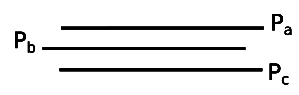
\includegraphics[width=4.5cm]{img/edge-clique.png} & &
    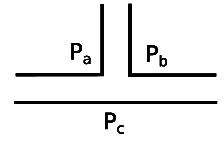
\includegraphics[width=3.5cm]{img/claw-clique.png}%b1EpgTransparenteGrade2
    \\
    \footnotesize %\centering 
    (a)  \footnotesize Representation of a clique as edge-clique. && \footnotesize (b) Representation  of a clique as claw-clique.\\
  \end{tabular}

 \caption{Examples of clique representations.} \label{fig:cliquesRepresentation}
\end{figure}

\section{Subclasses of Helly Graphs}

This paper starts with the following lemma.


\begin{lema} \label{lem:b1DiamondFree}
 If $G$ is a $B_1$-EPG and diamond-free graph then $G$ is a $B_1$-EPG-Helly graph.
 \end{lema}

\begin{pf}
If $G$ is not a $B_1$-EPG-Helly graph then in each $B_1$-EPG representation of $G$ there is at least one clique that is represented by claw-clique and no as edge-clique. Consider any of these  representations and let $K$ denote a clique in $G$ which is represented as a claw-clique. %If \mathcal{K} is part of a false or true pie
If there is a false or a true pie with the same center than the claw, then there is a 4-wheel graph ($W_4$) that has a diamond as induced subgraph and we are done.  Without loss of generality, we may assume that $K$ is maximal, and that the claw-clique has horizontal basis $[x_0, x_2]\times\{y_0\}$ and center $C = (x_1, y_0)$. Assume by \cite{ries2009}, without loss of generality, that no path $P_v, v\notin K$, uses the grid segment $[x_0, x_2]\times\{y_0\}$. Let us denote by  $\mathcal{K}$ the set of paths corresponding to the vertices of $K$. For every ${\displaystyle \lrcorner}$-path $P_v \in \mathcal{K}$ (resp. ${\displaystyle \llcorner}$-path $P_{v'} \in \mathcal{K}$), we do the following: if $P_v$ (resp. $P_{v'}$) does not intersect any path $P_w \notin \mathcal{K}$ on column $x_1$, then we delete its vertical segment and add the grid segment $[x_1, x_2]\times\{y_0\}$ (resp. $[x_0, x_2]\times\{y_0\}$). If after these transformations either there exist no more ${\displaystyle \lrcorner}$-paths in $\mathcal{K}$ or there exist no more ${\displaystyle \llcorner}$-paths in $\mathcal{K}$, then we are done since we have obtained an edge-clique. So we may assume that there exists at least one ${\displaystyle \lrcorner}$-path $P_v \in \mathcal{K}$ and at least one ${\displaystyle \llcorner}$-path $P_{v'} \in \mathcal{K}$. Since both paths $P_v, P_{v'}$ intersect a path on column $x_1$, they necessarily intersect a common path, say $P_t \notin \mathcal{K}$. Now if all ${\displaystyle \lrcorner}$-paths (resp. ${\displaystyle \llcorner}$-paths) do not intersect any path on row $y_0$, then we may transform them into ${\displaystyle \llcorner}$-paths (resp. ${\displaystyle \lrcorner}$-paths) with rightmost endpoint $(x_2,y_0)$ (resp. with leftmost endpoint $(x_0,y_0)$) and thus obtain an edge-clique. So we may assume that there exists at least one ${\displaystyle \lrcorner}$-path intersecting a path $P_{t'}\notin \mathcal{K}$ on row $y_0$ and there exists at least one ${\displaystyle \llcorner}$-path intersecting a path $P_{t''}\notin \mathcal{K}$ on row $y_0$. Without loss of generality, we may assume that $P_v$ intersects $P_{t'}$ and that $P_{v'}$ intersects $P_{t''}$. Clearly $P_{t'}$ and $P_{t''}$ cannot intersect since $t', t'' \notin K$ and all paths are single-bended. By the same arguments, $P_{t'}$, $P_{t''}$ cannot intersect $P_{t}$. But we are handling a claw-clique representation, then there is still at least a path $P_{u} \in \mathcal{K}$ on row $y_0$ that intersects $P_{v}$ and $P_{v'}$, necessarily, and $P_{u}$ may or may not intersect $P_{t'}$      and $P_{t''}$. But now $P_{v}, P_{v'}, P_{t}$ and $P_{u}$ induce a diamond, a contradiction.       
% Delimiters:
% \ulcorner	 
% \urcorner 
% \llcorner  {\displaystyle \llcorner }	\llcorner	 	{\displaystyle \lrcorner } {\displaystyle \lrcorner }	\lrcorner
  $\square$\end{pf}  

From the intersection model given in the proof of Lemma~\ref{lem:b1DiamondFree} we can to reconstruct the original graph, see Figure~\ref{fig:clawGrid}. This picture helps us to understand some constructions necessary for the existence of non-Helly structure in $B_1$-EPG graphs. In Figure~\ref{fig:clawGrid} the dashed edges are optional.


\begin{figure}
  \centering
  \begin{tabular}{  c p{0.7cm} c}
    %\centering
    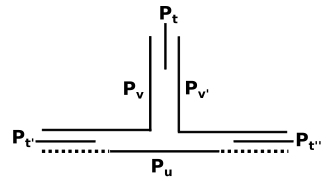
\includegraphics[width=5.5cm]{img/clawGrid} & &
    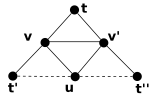
\includegraphics[width=3.5cm]{img/clawInduced.png}
    \\
    \footnotesize %\centering 
    (a)  \footnotesize Claw with paths. && \footnotesize (b) Subgraph induced by paths.\\
  \end{tabular}

 \caption{Reconstruction of the intersection model.}
 \label{fig:clawGrid}
\end{figure} 

 


The \textit{Cographs} are graphs whithout induced paths on four vertices, i.e. they are exactly the $P_4$-free graphs.


\begin{coro}
If $G$ is a Cograph $B_1$-EPG then $G$ $\in B_1$-EPG-Helly.
\end{coro}

\begin{pf}
Note that if there are edges $(P_{t'}$,$P_{u})$ and $(P_{t''}$,$P_{u})$ then there are many $P_4$'s and the representation is not Helly. Now if there are no edges $(P_{t'}$,$P_{u})$ and $(P_{t''}$,$P_{u})$ then the induced subgraph by set of vertices $\{P_{t'}, P_{v}, P_{v'}, P_{t''}\}$ forms a $P_4$. In other hand, cographs are graphs $P_4$-free, so if there are no paths of size 4 then there is no structures that requires claw-clique representation. %In other words when $G$ is cograph $P_{t'}$ and $P_{t''}$ cannot exist simultaneously in a single bend representation. 
Thus, every cograph $B_1$-EPG is Helly.
 $\square$\end{pf} 

\begin{coro}
If $G$ is a Bipartite $B_1$-EPG then $G$ is $B_1$-EPG-Helly.
\end{coro}

\begin{pf}
The Bipartite graphs are diamond-free, thus by Lemma~\ref{lem:b1DiamondFree} these graphs are $B_1$-EPG-Helly graphs.
\end{pf}


\begin{coro}\label{lem:cdf}
If $G$ is a Chordal and diamond-free graph then $G$ $ \in B_1$-EPG-Helly.
\end{coro}

\begin{pf}
The Theorema 19 from paper of \cite{ries2009} proved that diamond-free chordal graphs are all $B_1$-EPG, and by result of Lemma~\ref{lem:b1DiamondFree} of this paper we prove that when a graph is $B_1$-EPG and has no a diamond as subgraph then it is $B_1$-EPG-Helly, thus the Corollary hold.
 $\square$\end{pf} 

The Corollary~\ref{lem:cdf} expands and enriches the results from paper of \cite{ries2009}, so we delimit a proper subclass for the $B_1$-EPG-Helly graphs: the block graphs.

A \textit{block graph} or \textit{clique tree} is a type of graph in which every biconnected component (block) is a clique. These graphs also have a forbidden graph characterization as the graphs that do not have a diamond or a cycle of four or more vertices as an induced subgraph, i.e. block graphs = chordal $\cap$ diamond-free.

The problem of Block graph recognition is linear~\cite{tarjan1972depth}, so we know that at least one subclass of $B_1$-EPG-Helly has polynomial recognition. Since $B_1$-EPG-Helly recognition is a $\textsc{NP}$-complete problem, see~\cite{bornstein2019}.

% \begin{coro}
% Block (or Clique Tree) graphs are $B_1$-EPG-Helly graphs.
% \end{coro}

A \textit{Cactus} (sometimes called a cactus tree)  graph is a connected graph in which any two simple cycles have at most one vertex in common. Equivalently, it is a connected graph in which every edge belongs to at most one simple cycle, or (for nontrivial cactus) in which every block (maximal subgraph without a cut-vertex) is an edge or a cycle.
 
 The family of graphs in which each component is a cactus is downwardly closed under graph minor operations. This graph family may be characterized by a single forbidden minor, the four-vertex diamond graph formed by removing an edge from the complete graph $K_4$.
 
\begin{coro}
If $G$ is a Cactus $B_1$-EPG graph then $G$ $\in B_1$-EPG-Helly.
\end{coro}
\begin{pf}
Given a graph $G \in $ Cactus $B_1$-EPG. By definition, we know that $G$ is diamond-free, and by Lemma~\ref{lem:b1DiamondFree} we know that if a graph is $B_1$-EPG and diamond-free then this graph is  $B_1$-EPG-Helly. Therefore, by hypoteses $G$ is a $B_1$-EPG graph, thus $G$ is a $B_1$-EPG-Helly graph.
$\square$\end{pf}
 

 \begin{figure}[htb]	
 \center%6.3
 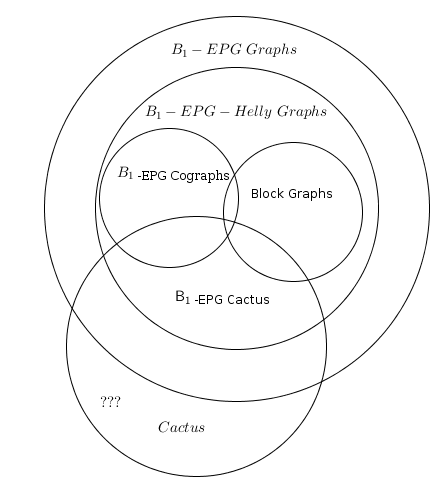
\includegraphics[width=7cm]{./img/DiagramaB1Helly.png}
 \caption{Diagram of some Helly graph classes}
\label{fig:diagram}
\end{figure}  
 

\begin{teo} (\cite{harary1974line})
A graph $G$ is a line-graph of a bipartite graph if and only if it
contains no claw, no odd hole, and no diamond.
\end{teo}


\begin{coro}
Let $G$ a $B_1$-EPG graph. If $G$ is a line graph of bipartite then $G \in B_1$-EPG-Helly. 
\end{coro}



Following we present some forbidden induced subgraphs for $B_1$-EPG paths whose representation is Helly, see Figure~\ref{fig:proibidos}.


\begin{figure}[h]
  \centering
  \begin{tabular}{  c p{0.7cm} c }
    \centering
    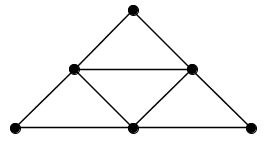
\includegraphics[width=4cm]{img/s3.png} & &
    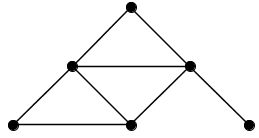
\includegraphics[width=4cm]{img/s3-1.png}
    \\
    \footnotesize \centering 
    (a)  \footnotesize Graph $S_3$ &&  \footnotesize (b) Graph $S_{3'}$ \\
    
    %---------------------
      \centering 
      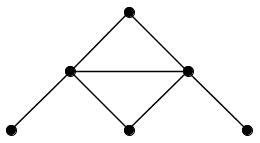
\includegraphics[width=4cm]{img/s3-2.png} & &
    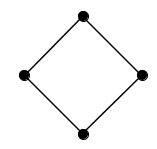
\includegraphics[width=3cm]{img/c4.png}
    \\
    \footnotesize \centering 
    (c)  \footnotesize Graph $S_{3''}$ && \footnotesize (b) Graph $C_{4}$\\
  \end{tabular}

 \caption{Set of subgraphs that define a  $B_1$-EPG-Helly subfamily}
 \label{fig:proibidos}
\end{figure} 


\begin{coro}
\label{lem:chordalDiamondFree}
Let $G$ a $B_1$-EPG graph. If $G$ is  $\{S_{3}, S_{3'}, S_{3''}, C_{4}\}$-free then $G$  $\in B_1$-EPG-Helly.
\end{coro}
%--------------------------

% \begin{defi}
% We say that $T_1, T_2$ are \textbf{rooted trees by paths of the maximal edge-clique} $k$ when occur:
% \begin{itemize}
%     \item there are points $q_1, q_2$, respectively leftmost and rightmost (w.l.g. above and below) where all paths of $k$ meet;
%     \item $T_1, T_2$ are collections of grid edges that do not belong to edge-clique $k$ but belong to paths of $k$ and are rooted, respectively, in $q_1, q_2$. Furthermore, the trees $T_1, T_2$ are disjoint.
    
%     %\item $T_1, T_2$ are trees rooted, respectively, in $q_1, q_2$ and formed by each path that does not belong to clique $k$ but intersects to some path of $k$;
% \end{itemize}
% \end{defi}

% \begin{defi}
% Let $T_i$ be a rooted tree by paths of the maximal edge-clique $k$, we say that a path $P_j$ is an \textbf{aggregate} from the tree $T_i$ if it intersects any edge of $T_i$.
% \end{defi}

\section{Subclasses of EPT graphs }

In this section we will present sufficient conditions to show that a given graph $B_1$-EPG belongs to VPT and EPT. In the following text we insert some useful definitions for the next demonstrations.

\begin{defi}
  A \textbf{satellite} of a clique $C$ is a vertex $v$ such that $B_v=N(v)\cap C$ is a 
nonempty proper subset of $C$. The set $B_v$ is called the base of $v$ and it is said minimal if no other
base of a satellite of $C$ is properly contained in $B_v$.
\end{defi}


\begin{defi}
 Let $I=[q_1,q_2]$ be the grid interval defined by the intersection $\cap_{v\in C}P_v$, where $C$
is an edge-clique of a graph $G$. For any $v\in C$, by removing the interval $(q_1,q_2)$, the path $P_v$
is split into to disjoint parts: part 1  containing $q_1$, and  part 2  containing $q_2$.
If $w$  is a satellite of $C$ adjacent to $v$, then
$P_w\cap P_v$ is contained either in part 1 or in part 2 of $P_v$. We will say that $P_w$ intersects $P_v$
on side 1 or on side 2 of $C$, respectively. Notice that if $w$  is also adjacent
to another vertex $v'$ of $C$, then   $P_w$ intersects $P_v$ and $P_{v'}$ on
a same side of $C$. It allow us to divide the satellites of $C$ into two disjoint
groups, the ones on  side 1 of $C$ and the ones on side 2.
\end{defi}

% \begin{defi}
% We say that a $B_1$-EPG representation $R'$ is a \textbf{partial representation} of other $B_1$-EPG representation $R$ if $R' \subseteq R$.
% \end{defi}

\begin{lema}\label{lem:3cliquesNotClaw}
Let $G$ be a graph whose vertex set  can be
partitioned into a non trivial clique $K=\{u_1,\ldots,u_k\}$ and a independent set $I=\{w_1,w_2,w_3\}$, such that each vertex of $K$ is adjacent to each vertex of $I$ and where each subset $C_i = K \cup w_i$ is a different maximal clique. At least one $C_i$ is edge-clique. 
\end{lema}

\begin{pf}
Given $\mathcal{P}_K, \mathcal{P}_I$ the set paths representing vertices of $K$ and $I$, respectively. 
Suppose there is a representation in which each maximal clique $K \cup \{w_i\}$ is represented by claw-clique, respectively $C_1, C_2, C_3$. $\mathcal{P}_K$ can not be part only of base in each $C_i$ because each $P_i \in \mathcal{P}_I$ was one only path with bend in each claw-clique. Thus each claw-clique $C_i$ has at least one path $P_k \in \mathcal{P}_K$ that bend in this claw-clique. If all paths $P_k \in \mathcal{P}_K$ bend in some claw-clique then these paths can not bend in other claw-clique, i.e. if all paths $P_k \in \mathcal{P}_K$ bend in some claw-clique others cliques will be edge-clique and Lemma holds. Maybe that at least one path $P_k \in \mathcal{P}_K$ has bend and at least one another different path $P_k \in \mathcal{P}_K$ has no bend in each $C_i$. In this way, in each claw-clique $C_i$, or all paths $P_k \in \mathcal{P}_K$ intersect in some segment between center of claw-clique and right or left part of base, or then there is only one point of intersection of all paths (center of this claw, obviously) and there is no a $B_1$-EPG representation to $G$. Consider first situation,  w.l.g. we say that claw-clique $C_1$ has base in interval $(q_1,q_2)$ and that all paths $P_k \in \mathcal{P}_K$ are  at right to $q_2$. Then other claw-clique $C_3$ with base in interval $(q_1'',q_2'')$ has same condition but with intersection of all paths at left of $q_1''$. Now, we have a problem, in claw-clique $C_2$ with base in interval $(q_1',q_2')$ the paths $P_k \in \mathcal{P}_K$ can not participate simultaneously to the right of the base of cliques $C_1$ and $C_2$, nor to the left of clicks $C_2$ and $C_3$. Therefore at least one clique in this construction is edge-clique.
\end{pf}


\begin{coro}\label{coro:3Cliques1EdgeClique}
In any $B_1$-EPG representation of $G$ there is at least one edge-clique $C_i$ that is located between two satellites $w_i$.
\end{coro}



%-----------------------------------------------------
\begin{lema} \label{lem:obstrucaoCentro}
%Let $C_{B}$ be the graph of Figure~\ref{fig:obstrucaoCentro}. Let $C_{B'}$ be the subgraph of the graph $C_{B}$ where  $C_{B'} = C_{B} -\{n\}$. Let $R'$ be a $B_1$-EPG representation of $C_{B'}$, where the clique $C=\{a,b,2\}$ is represented by edge-clique. If when we take $T_1, T_2$, rooted trees by paths of the maximal edge-clique $C$, occur that paths $P_{1}$ and $P_{3}$ are not aggregates of the same tree, then there is no $B_1$-EPG representation of $C_{B}$ whose $R'$ is its $B_1$-EPG partial representation.
Let $C$ be the edge-clique $\{a,b,2\}$ of the graph $C_B$ on Figure~\ref{fig:obstrucaoCentro}.
In any $B_1$-EPG representation $R$ of $C_{B}$  the satellites $1$ and $3$
are on the same side of $C$.
\end{lema}

\begin{pf}
By Lemma~\ref{lem:3cliquesNotClaw} the maximal cliques $C_1, C_2$ and $C_3$ can not be simultaneously by claw-clique and by Corollary~\ref{coro:3Cliques1EdgeClique} there is one edge-clique $C_i$ whose 2 paths representing satellites of independent set $I$ are in different sides of  $C_i$. Thus if w.l.g. $C_1$ is represented by claw-clique then $C_2$ and $C_3$ are of same side of $C_1$.


Let $C_{B'}$ be the subgraph obtained by $C_{B}-\{n\}$ and $R'$ its $B_1$-EPG representation, where the satellites $1$ and $3$ are in disjoint groups relative to edge-clique $C$. 
 We know that in $C_{B'}$ occur  $N(1) = N(2) = N(3)$. The path $P_{2}$ is on edge-clique $C$ and it is between  $P_{1}$ and $P_{3}$. % whether we consider the edge-clique $C$. 
 Thus it will not be possible to insert the path $P_{n}$ intersecting only $P_{b}$ and $P_{2}$ in single bend. However there is no $B_1$-EPG representation of $C_{B}$ such that $R' \subset R$. $\square$
 \begin{figure}[htb]	
 \center%6.3
 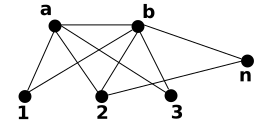
\includegraphics[width=5cm]{./img/obstrucaoCentro.png}
 \caption{Graph Center Blocked $C_B$}
\label{fig:obstrucaoCentro}
\end{figure}  
 
 \end{pf} 

Now, we will construct $C_{B''}$ composited by 3 subsets: $K=\{a,b\}$, $I_1=\{w_1,w_2,w_3\}$  and
$I_2=\{1,2,3\}$, such that each vertex of $K$ is adjacent to each vertex of $I_1$, and each  $i\in I_2$ is adjacent to $w_i\in I_1$ and to a proper subset $S_i$ of $K$. In addition, $I_2$ elements may or may not have edges with each other.

%. We will say $K=\{a, b\}$, $I=\{1, 2,3\}$ and $R=\{n-1, n,  n+1\}$, where each element of $R$ is adjacent only element of $I$  %with adjacencies $\{({n-1},1); ({n-1},k); ({n+1},3), ({n+1},k)\}$, where $k \in K$.

\begin{lema}\label{lem:cb''}
The graph $C_{B''}$  $\notin B_1$-EPG.
\end{lema}

\begin{pf}
Since the elements of $I_1$ form a independent set with adjacencies to the vertices $a,b$, then at least one clique $C = \{a,b,w_i\}$, where $w_i \in I_1$ is represented by edge-clique. If others two cliques are claw-clique then this edge-clique is between these claw-cliques and by Lemma~\ref{lem:obstrucaoCentro} this construction does  not have a $B_1$-EPG representation. Yet if only one clique $C$ is represented by claw-clique, others two cliques $C$ are represented by edge-clique and one of these edge-cliques is at case of Lemma~\ref{lem:obstrucaoCentro} and again this construction does  not have a $B_1$-EPG representation. %Yet that in the claw-clique $P_{a}$ and $P_{b}$ be paths of the type ${\displaystyle \llcorner}$-path and ${\displaystyle \lrcorner}$-path, or ${\displaystyle \llcorner}$-path (resp. ${\displaystyle \lrcorner}$-path) and ${\displaystyle -}$-path both cases will always exists one edge-clique like in Lemma~\ref{lem:obstrucaoCentro}. 
The case where the 3 cliques $C$ are represented by edge-clique is trivial and also solved by Lemma~\ref{lem:obstrucaoCentro}.
 $\square$\end{pf} 

A generalization of the Lemmata~\ref{lem:obstrucaoCentro} and \ref{lem:cb''} is presented to follow.

\begin{lema}\label{lem:obstrucaoGeneralizada}
Let $G$ be a graph whose vertex set  can be
partitioned into a non trivial clique $K=\{u_1,\ldots,u_k\}$, a independent set $I_1=\{w_1,w_2,w_3\}$  and
$I_2=\{1,2,3\}$, such that each vertex of $K$ is adjacent to each vertex of $I_1$, and each  $i$ is adjacent to $w_i$ and to a proper subset $S_i$ of $K$. In addition, $I_2$ elements may or may not have edges with each other.
%Let $G$ be the graph with  the following distinct sets of vertices, $K=\{u_1, \dots, u_k\}$, where $K$ is a clique and $|K|\geq 2$; $I_1 =\{w_1,w_2,w_3 \}$, where $I_1$ is an  independent set and there is  $K \Join I_1$; $I_2 =\{ \forall w_i \in I_1 \exists !i \in I_2 | (w_i, i), \textrm{ if } i\neq i' \textrm{ then } i \neq {i'}\}$, where  $ \forall i \in I_2 \exists \cup\{(i,u_j)\}$, such that $1\leq |\cup\{(i,u_j)\}| \leq k-1$. The graph $G$ is not a $B_1$-EPG graph.
%, such that the vertices of $k$ are a clique and the vertices of $I_1$ and $I_2$ are independent sets. 
\end{lema}

\begin{pf}
Since the elements of $I_1$ form a independent set, at least one $w_i \in I_1$ is represented by edge-clique with paths of $K$, and as others two elements are claw-clique with same elements of $K$, so this edge-clique is between these claw-cliques and by Lemma~\ref{lem:obstrucaoCentro} there is not a valid $B_1$-EPG representation for this construction. Yet if only one $w_i\in I_1$ is represented by claw-clique with elements of $k$, others two cliques are represented by edge-cliques and one of these edge-cliques is in case of Lemma~\ref{lem:obstrucaoCentro} and again there is not a valid $B_1$-EPG representation for this construction. 
The case where the 3 cliques with $K$ are represented by edge-clique is trivial and also solved by~Lemma~\ref{lem:obstrucaoCentro}. In any cases a construction of a $B_1$-EPG representation for $G$ is not possible.
 $\square$\end{pf}

%--------------------------

% \begin{defi}
% Considering a claw-clique with horizontal base, without loss of generality, we can say that a claw-clique has 3 distinct paths types:
% \begin{itemize}
%     \item ${\displaystyle \llcorner}$-path;
%     \item ${\displaystyle \lrcorner}$-path;
%     \item ${\displaystyle -}$-path.
% \end{itemize}
% \end{defi}

\begin{lema}\label{lem:cliquesMaximais}
%If $P_a, P_b, P_c$ form a claw in a $B_1$-EPG representation then the vertices $a, b, c$ are together in a unique maximal clique of $G$.
If three vertices are together  in more than one maximal clique of a graph $G$, then in
any $B_1$-EPG representation of $G$ the corresponding paths do not form a claw.
\end{lema}

\begin{pf}
Let $(x_0,x_1), (x_1,y_1), (x_1,x_2) $ be the central edges of the claw formed by $P_a, P_b$ and $P_c$. Any path intersecting $P_a, P_b$ and $P_c$ has 2 of these edges, since the proof follows, see Figure~\ref{fig:lemaClaw2Maximais}.
%Suppose that $P_a, P_b, P_c$ are paths of two maximal cliques, $C_1$ and $C_2$, the first with path $P_1 \in C_1 - C_2$ and the second with the path $P_2 \in C_2 - C_1$. Suppose that the base of claw-clique is horizontal and the center is on $(x_0, y_0)$. As $P_1, P_2$ are paths of distinct maximal cliques then both $P_1, P_2$ belong to claw-clique and $P_1 \cap P_2 \neq \emptyset$, absurd. 
 %If $P_1$ and $P_2$ belong to $C$ then $P_1$ and $P_2$ are paths of type ${\displaystyle \llcorner}$-path, ${\displaystyle \lrcorner}$-path or ${\displaystyle -}$-path. If $P_1$ and  $P_2$ are both the same type, if they are of types ${\displaystyle \llcorner}$-path and ${\displaystyle \lrcorner}$-path, or if one is type ${\displaystyle -}$-path and the other is type ${\displaystyle \llcorner}$-path or ${\displaystyle \lrcorner}$-path, then in each case $P_1 \cap P_2 \neq \emptyset$, this is a contradiction with fact $P_1$ and $P_2$ belong to maximal cliques distinct.
 $\square$\end{pf} 

%  \begin{figure}[htb]	
%  \center%6.3
%  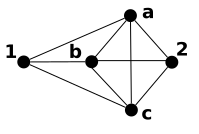
\includegraphics[width=5cm]{./img/lemaClaw2Maximais.png}
%  \caption{Example of Construction 1 }
% \label{fig:lemaClaw2Maximais}
% \end{figure}  
 
 
 
\begin{figure}[ht]
  \centering
  \begin{tabular}{  p{5cm} p{0.7cm} p{5cm} }
    %\centering
    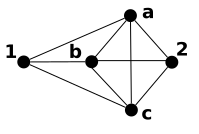
\includegraphics[width=3.5cm]{img/lemaClaw2Maximais} & &
    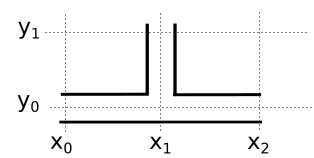
\includegraphics[width=5.5cm]{img/claw2}
    \\
    \footnotesize %\centering 
    (a)  \footnotesize Example of two maximal cliques sharing vertices. && \footnotesize (b) Representation  of a claw-clique in grid.\\
  \end{tabular}

 \caption{Vertices represented by a claw are present in a unique maximal clique.} \label{fig:lemaClaw2Maximais}
\end{figure}

% \begin{lema}\label{lem:clawNotPossible}
% Given a claw-clique $C$ of a chordal graph $G$, in a $B_1$-EPG representation, given paths $P_a, P_b, P_c$ respectively of type ${\displaystyle \lrcorner}$-path, ${\displaystyle \llcorner}$-path and ${\displaystyle -}$-path, where $P_a, P_b, P_c \in C$. Let $P_1, P_6, P_7, P_8$ be paths where must there are the following intersections: $\{P_1 \cap P_a\}$, $\{P_1 \cap P_b\}$, $\{P_6 \cap P_a\}$, $\{P_6 \cap P_b\}$, $\{P_6 \cap P_c\}$, $\{P_6 \cap P_7\}$, $\{P_7 \cap P_a\}$, $\{P_7 \cap P_b\}$, $\{P_7 \cap P_8\}$, $\{P_8 \cap P_b\}$, then there is no a valid $B_1$-EPG representation to this set of intersections.
% \end{lema}

% \begin{figure}[htb]	
 \center%6.3
 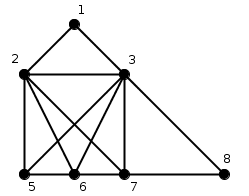
\includegraphics[width=5cm]{./img/grafoH.png}
 \caption{Graph $H$}
\label{fig:grafoH}
\end{figure}  
 

In paper of~\cite{alcon2015characterizing}, the authors define a family of minimal forbidden induced subgraphs for VPT graphs. They present 17 forbidden induced subgraphs for VPT graphs, see Figure~\ref{fig:16proibidos}. We are interested in the 16 graphs that are Chordal, so let is discard the cycle $C_n, n\geq4$. Now we will study how constructions of each of these graphs occur in $B_1$-EPG representations.


 \begin{figure}[htb]	
 
   \centering
  \begin{tabular}{  c c c c  c}
    %\centering
    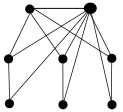
\includegraphics[width=2.5cm]{img/f1.png} 
    & 
    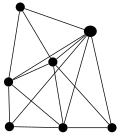
\includegraphics[width=2.3cm]{img/f2.png} 
    & 
    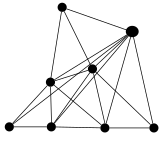
\includegraphics[width=3cm]{img/f3.png} 
    & 
    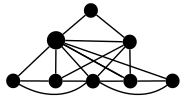
\includegraphics[width=3cm]{img/f4.png} 
    & 
    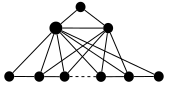
\includegraphics[width=3cm]{img/f5.png} 
    \\
    \footnotesize 
    (a)  \footnotesize Graph $F_1$. 
    & 
    \footnotesize (b) Graph $F_2$.
    & 
    \footnotesize (c) Graph $F_3$.
    & 
    \footnotesize (d) Graph $F_4$.
    & 
    \footnotesize (e) Graph $F_5(n),n\geq7$.
    \\%%Segunda linha
        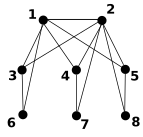
\includegraphics[width=2.5cm]{img/f6.png} 
    & 
    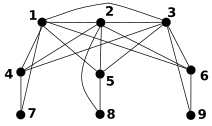
\includegraphics[width=3.5cm]{img/f7.png} 
    & 
    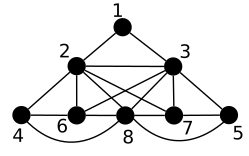
\includegraphics[width=3cm]{img/f8.png} 
    & 
    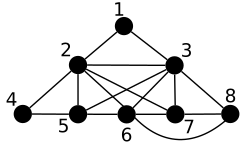
\includegraphics[width=3cm]{img/f9.png} 
    & 
    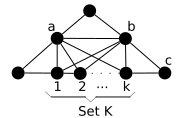
\includegraphics[width=3cm]{img/f10n.png} 
    \\ %%Segundo Bloco legendas
    \footnotesize 
    (f)  \footnotesize Graph $F_6$. 
    & 
    \footnotesize (g) Graph $F_7$.
    & 
    \footnotesize (h) Graph $F_8$.
    & 
    \footnotesize (i) Graph $F_9$.
    & 
    \footnotesize (j) Graph $F_{10}(n), n\geq  8$.
    %%Terceira linha de imagens
    \\%%Terceira linha
        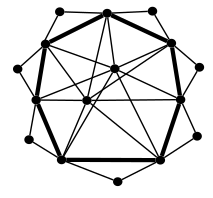
\includegraphics[width=3cm]{img/f11.png} 
    & 
    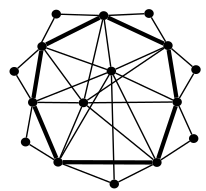
\includegraphics[width=3cm]{img/f12.png} 
    & 
    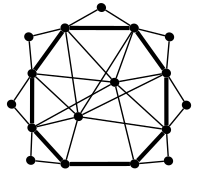
\includegraphics[width=3cm]{img/f13.png} 
    & 
    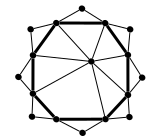
\includegraphics[width=3cm]{img/f14.png} 
    & 
    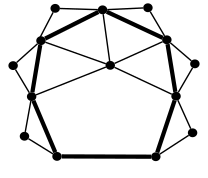
\includegraphics[width=3cm]{img/f15.png} 
    \\ %%Terceiro Bloco legendas
    \footnotesize 
    (k)  \footnotesize  $F_{11}(4k),k\geq2$. 
    & 
    \footnotesize (l)  $F_{12}(4k),k\geq2$.
    & 
    \footnotesize (m)  $F_{13}(4k+1),k\geq2$.
    & 
    \footnotesize (n)  $F_{14}(4k+1),k\geq2$.
    & 
    \footnotesize (o)  $F_{15}(4k+2),k\geq2$.
    
    \\ %Ultima linha Figuras
    
    && 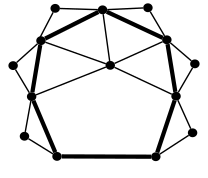
\includegraphics[width=3cm]{img/f15.png} &&
    
    \\%Ultima linha Legendas
    
    && \footnotesize (p)  $F_{16}(4k+3),k\geq2$. &&
    
    %\multicolumn{3}{c}{ \footnotesize (c) Another partial single bend representation of $H$ } \\
  \end{tabular}
 \caption{The 16 Chordal induced subgraphs forbidden to VPT (the vertices in the cycle marked by bold edges form a clique).}
 %, see  more in~\cite{leveque2009characterizing,tondato2009grafos}
 \label{fig:16proibidos}
\end{figure}  
 


% \begin{lema}\label{lem:clawNotPossible235}
% In any $B_1$-EPG representation of the graph $H$, see Figure~\ref{fig:noClawVertical}(a), paths $P_2, P_3, P_5$ do not form a claw.
% \end{lema}

% \begin{pf}
% Suppose that paths $P_2, P_3, P_5$ are  respectively of type ${\displaystyle \lrcorner}$-path, ${\displaystyle \llcorner}$-path and ${\displaystyle -}$-path, see Figure~\ref{fig:noClawVertical}(b). Without less of generality, we consider claw-clique with center $(x_1, y_0)$ and base on row $y_0$.
% The paths $P_2$, $P_3$ and $P_6$ are in two maximal cliques ($\{$ $P_6$,$P_2$,$P_3$,$P_5$  $\}$ and $\{$ $P_6$,$P_2$,$P_3$,$P_7$ $\}$), thus by Lemma~\ref{lem:cliquesMaximais} then $P_6$ is represented like edge-clique with $P_2$ and $P_3$. This way $P_6$ has segment on column $x_1$ intersecting $P_2$ and $P_3$ and with bend at row $y_0$ to intersects $P_5$. The path $P_1$ has intersection only with $P_2$ and $P_3$ then $P_1$ has segment on column $x_1$ above last segment of intersection of $P_6 \cap$ $P_2 \cap$ $P_3$.  The path $P_7$ is intersecting  $P_6 \cap$ $P_2 \cap$ $P_3$  and no $P_1$ and $P_5$ then  it is on column $x_1$ and not on row $y_0$. But there is the path $P_8$ that also intersects $P_7$ and $P_3$. Now, path $P_7$ cannot bend in row $y_0$ because it does not intersect $P_5$, in other hand it cannot to extend on column $x_1$ to find any place where occur intersection with $P_8$ and $P_3$. As $P_3$ already has bend, $P_7$ is blocked in column $x_1$ by $P_1$ and $P_7$ cannot bend in row $y_0$  so it is not possible to put in a path $P_8$ intersecting  only at $P_3$ and $P_7$, see Figure~\ref{fig:noClawVertical}(b). 

%  \begin{figure}[htb]	
 
   \centering
  \begin{tabular}{  c p{0.7cm} c}
    %\centering
    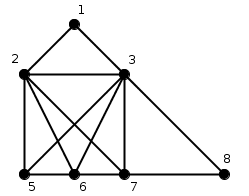
\includegraphics[width=5cm]{img/grafoH.png} & &
    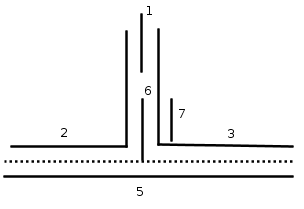
\includegraphics[width=5cm]{img/noClawVertical.png}
    \\
    \footnotesize %\centering 
    (a)  \footnotesize Graph $H$ && \footnotesize (b) Partial single bend representation of $H$\\
    \multicolumn{3}{c}{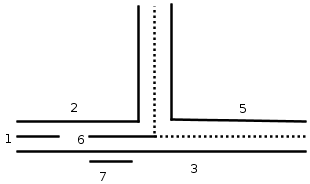
\includegraphics[width=5cm]{img/noClawHorizontal.png}  }
    \\
    \multicolumn{3}{c}{ \footnotesize (c) Another partial single bend representation of $H$ }
    \\
  \end{tabular}
 \caption{Graph $H$ and a partial constructions on single bend}
%  \center%6.3
%  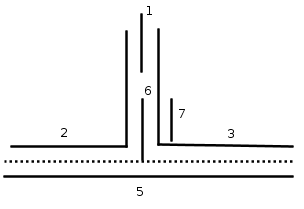
\includegraphics[width=5cm]{./img/noClawVertical.png}
%  \caption{Example of Construction 2 }
 \label{fig:noClawVertical}
\end{figure}  
 

% Thus, if there is some  $B_1$-EPG representation for $H$ where  paths $P_2, P_3, P_5$ are represented by claw-clique, then in this representation  $P_5$ is not of type ${\displaystyle -}$-path.


% Now suppose that paths $P_2, P_5, P_3$ are  respectively of type ${\displaystyle \lrcorner}$-path, ${\displaystyle \llcorner}$-path and ${\displaystyle -}$-path, see Figure~\ref{fig:noClawVertical}(c). By Lemma~\ref{lem:cliquesMaximais} we know that the clique formed by $P_2$, $P_3$ and $P_6$ is represented like edge-clique. This way $P_6$ has segment on row $y_0$ intersecting $P_2$ and $P_3$ and $P_6$ can bend on column $x_1$ or make part to base on row $y_0$ to intersect $P_5$. The path $P_1$ has intersection only with $P_2$ and $P_3$, then $P_1$ has segment on row $y_0$ to left last segment of intersection of $P_2 \cap$ $P_3 \cap$ $P_6$.  The path $P_7$ is intersecting  $P_2 \cap$ $P_3 \cap$ $P_6$ and no $P_1$ and $P_5$ then it is on row $y_0$, but there is the path $P_8$ that also intersects $P_3$ and $P_7$. Now, path $P_7$ cannot cross the center of claw-clique because it does not intersect $P_5$, in other hand it cannot to extend on row $y_0$ to find any place where occur intersection with $P_3$ and $P_8$, this because $P_7$ is blocked in row $y_0$ by $P_1$ and $P_5$. The path $P_3$ could bend only one edge after of the center of claw-clique, or forming another claw-clique with $P_1$ and $P_2$, or yet before of intersection $P_1 \cap$ $P_2 \cap$ $P_3$, but in each case is not possible to put in a path $P_8$ intersecting  only at $P_3$ and $P_7$, see Figure~~\ref{fig:noClawVertical}(c).

% Again we find a new condition of existence for some  $B_1$-EPG representation to $H$ where  paths $P_2, P_3, P_5$ are represented by claw-clique. If there is this representation then  $P_3$ is not of type ${\displaystyle -}$-path. But note that if paths paths $P_3, P_5, P_2$ are  respectively of type ${\displaystyle \lrcorner}$-path, ${\displaystyle \llcorner}$-path and ${\displaystyle -}$-path, then claw-clique intersections continue to occur as in the previous case and the same constraints remain valid.

% Therefore, we can conclude that there is not a $B_1$-EPG representation of the graph $H$ where $P_2, P_3,$ $P_5$ are represented by claw-clique.
%  $\square$\end{pf} 

% \begin{lema}\label{lem:clawNotPossible256}
% In any $B_1$-EPG representation of the graph $k$-tent, see Figure~\ref{fig:ktent}, paths $P_2, P_5, P_6$ do not form a claw.
% \end{lema}

% \begin{pf}
% Suppose that paths $P_2, P_5, P_6$ are  respectively of type ${\displaystyle \lrcorner}$-path, ${\displaystyle \llcorner}$-path and ${\displaystyle -}$-path. Without less of generality, we consider claw-clique with center $(x_1, y_0)$ and base on row $y_0$.
% The paths $P_2$, $P_3$ and $P_6$ are in two maximal cliques ($\{$ $P_6$,$P_2$,$P_3$,$P_5$  $\}$ and $\{$ $P_6$,$P_2$,$P_3$,$P_7$ $\}$), thus by Lemma~\ref{lem:cliquesMaximais} then $P_6$ is represented like edge-clique with $P_2$ and $P_3$. This way $P_3$ has segment on row $y_0$ intersecting $P_2$ and $P_6$ and with bend at column $x_1$ or cross center of claw-clique to intersects $P_5$. The path $P_4$ has intersection only with $P_2$ and $P_5$, then there is segment of $P_2 \cap$ $P_4 \cap$ $P_5$ on column $x_1$, because $P_4$ does not intersect $P_6$.
% The path $P_1$ has intersection only with $P_2$ and $P_3$ then $P_1$ has segment on row $y_0$ and  Next, the path $P_7$ is intersecting  $P_6 \cap$ $P_2 \cap$ $P_3$ then maybe it is on row $y_0$ between some segment of $P_1$ and center of claw-clique, but yet there is the path $P_8$ that also intersects $P_7$ and $P_3$. Now, path $P_7$ cannot bend in column $x_1$ because it does not intersect $P_5$, in other hand it cannot to extend on row $y_0$ to find any place where occur intersection with $P_3$ and $P_8$. The path $P_7$ is blocked in row $y_0$ by $P_1$ and $P_5$. The path $P_3$ can bend after of center claw-clique or bending with $P_1$ both cases are not possible to put in a path $P_8$ intersecting  only at $P_3$ and $P_7$, see Figure~\ref{fig:noClaw256}(a). 

%  \begin{figure}[htb]
 
  \centering
  \begin{tabular}{  c p{0.7cm} c}
    %\centering
    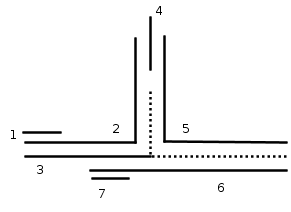
\includegraphics[width=5cm]{img/noClaw256.png} & &
    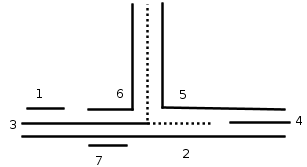
\includegraphics[width=5.2cm]{img/noClaw652.png}
    \\
    \footnotesize %\centering 
    (a)  \footnotesize Claw-clique $P_2$, $P_5$, $P_6$ && \footnotesize (b) Claw-clique $P_6$, $P_5$, $P_2$\\
    \multicolumn{3}{c}{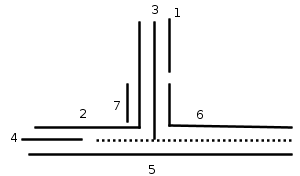
\includegraphics[width=5cm]{img/noClaw265.png}  }
    \\
    \multicolumn{3}{c}{ \footnotesize (c) Claw-clique $P_2$, $P_6$, $P_5$ }
    \\
  \end{tabular}
 
%  \center%6.3
%  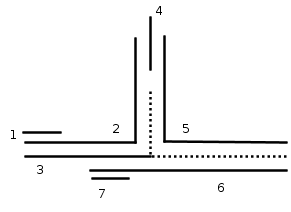
\includegraphics[width=5cm]{./img/noClaw256.png}
 \caption{Constructions in single bend of $k$-tent with $P_2$, $P_5$ and $P_6$ in claw-clique representation }
\label{fig:noClaw256}
\end{figure}  
 

% Thus, if there is some  $B_1$-EPG representation for $k$-tent where  paths $P_2, P_5, P_6$ are represented by claw-clique, then in this representation  $P_6$ is not of type ${\displaystyle -}$-path.  Note yet that if paths paths $P_6, P_5, P_2$ are  respectively of type ${\displaystyle \lrcorner}$-path, ${\displaystyle \llcorner}$-path and ${\displaystyle -}$-path, then claw-clique intersections continue to occur as in the previous case and the same constraints remain valid, see Figure~\ref{fig:noClaw256}(b). Thus we know that in this representation  $P_2$ is not of type ${\displaystyle -}$-path. Therefore, we only need to analyze one more configuration. 

% %%%%%%%%%%%%%%%%%%%%%
% Now suppose that paths $P_2, P_6, P_5$ are  respectively of type ${\displaystyle \lrcorner}$-path, ${\displaystyle \llcorner}$-path and ${\displaystyle -}$-path. By Lemma~\ref{lem:cliquesMaximais} we know that the clique formed by $P_2$, $P_3$ and $P_6$ is represented like edge-clique. This way $P_3$ has segment on column $x_1$ intersecting $P_2$ and $P_6$ and bending on row $y_0$  to intersect $P_5$. The path $P_1$ has intersection only with $P_2$ and $P_3$ then $P_1$ has segment on column $x_1$. The path $P_4$ intersects $P_2$ and $P_5$ on row $y_0$.  The path $P_7$ is intersecting  $P_2 \cap$ $P_3 \cap$ $P_6$ then maybe it is on column $x_1$ between $P_1$ and center of claw-clique, but there is the path $P_8$ that also intersects $P_3$ and $P_7$. Now, path $P_7$ cannot cross the center of claw-clique because it does not intersect $P_5$, in other hand it cannot to extend on column $x_1$ to find any place where occur intersection with $P_3$ and $P_8$, this because $P_7$ is blocked on column $x_1$ by $P_1$ and  in row $y_0$ by $P_5$. The path $P_3$ could bend only one edge after of the center of claw-clique, or forming another claw-clique with $P_1$ and $P_2$, or yet before of intersection $P_1 \cap$ $P_2 \cap$ $P_3$, but in each case is not possible to put in a path $P_8$ intersecting  only at $P_3$ and $P_7$, see Figure~\ref{fig:noClaw256}(c).
% %Again we find a new condition of existence for some  $B_1$-EPG representation to $H$ where  paths $P_2, P_3, P_5$ are represented by claw-clique. If there is this representation then  $P_3$ is not of type ${\displaystyle -}$-path. But note that if paths paths $P_3, P_5, P_2$ are  respectively of type ${\displaystyle \lrcorner}$-path, ${\displaystyle \llcorner}$-path and ${\displaystyle -}$-path, then claw-clique intersections continue to occur as in the previous case and the same constraints remain valid.
% %Therefore, we can conclude that there is not a $B_1$-EPG representation of the graph $H$ where $P_2, P_3,$ $P_5$ are represented by claw-clique.
%  $\square$\end{pf} 

% \begin{lema}\label{lem:clawNotPossible356}
% In any $B_1$-EPG representation of the graph $H$, see Figure~\ref{fig:noClawVertical}(a), paths $P_3, P_5, P_6$ do not form a claw-clique.
% \end{lema}

% \begin{pf}
% Suppose that paths $P_3, P_6, P_5$ are  respectively of type ${\displaystyle \lrcorner}$-path, ${\displaystyle \llcorner}$-path and ${\displaystyle -}$-path. Without less of generality, we consider claw-clique with center $(x_1, y_0)$ and base on row $y_0$.
% The vertices $2$, $3$ and $6$ are in two maximal cliques ($\{$ $6$,$2$,$3$,$5$  $\}$ and $\{$ $6$,$2$,$3$,$7$ $\}$), thus by Lemma~\ref{lem:cliquesMaximais} then $P_2$ is represented like edge-clique with $P_3$ and $P_6$. This way $P_2$ has segment on column $x_1$ intersecting $P_3$ and $P_6$ and with bend at row $y_0$ to intersects $P_5$. The Intersection $P_2 \cap P_4 \cap P_5$ has at least one segment on row $y_0$. The path $P_1$ has intersection only with $P_2$ and $P_3$ then $P_1$ has segment on column $x_1$ above last segment of intersection of $P_6 \cap$ $P_2 \cap$ $P_3$.  The path $P_7$ is intersecting  $P_6 \cap$ $P_2 \cap$ $P_3$ then maybe it is on column $x_1$, but there is the path $P_8$ that also intersects $P_7$ and $P_3$. Now, path $P_7$ cannot bend in row $y_0$ because it does not intersect $P_5$, in other hand it cannot to extend on column $x_1$ to find any place where occur intersection with $P_8$ and $P_3$. As $P_3$ already has bend, $P_7$ is blocked in column $x_1$ by $P_1$ and $P_7$ cannot bend in row $y_0$  so it is not possible to put in a path $P_8$ intersecting  only at $P_3$ and $P_7$, see Figure~\ref{fig:noClaw365}(a). 

%  \begin{figure}[htb]
 
  \centering
  \begin{tabular}{  c p{0.7cm} c}
    %\centering
    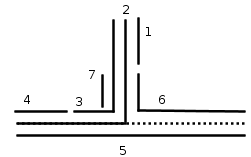
\includegraphics[width=5cm]{img/noClaw365.png} & &
    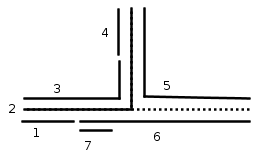
\includegraphics[width=5.2cm]{img/noClaw356.png}
    \\
    \footnotesize %\centering 
    (a)  \footnotesize Claw-clique $P_3$, $P_6$, $P_5$ && \footnotesize (b) Claw-clique $P_3$, $P_5$, $P_6$\\
    \multicolumn{3}{c}{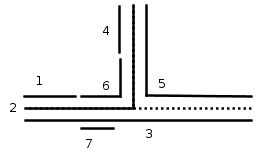
\includegraphics[width=5cm]{img/noClaw653.png}  }
    \\
    \multicolumn{3}{c}{ \footnotesize (c) Claw-clique $P_6$, $P_5$, $P_3$ }
    \\
  \end{tabular}
 
%  \center%6.3
%  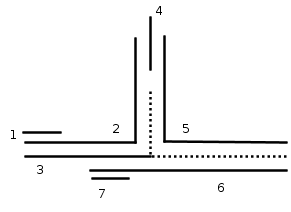
\includegraphics[width=5cm]{./img/noClaw256.png}
 \caption{Constructions in single bend of $k$-tent with $P_3$, $P_5$ and $P_6$ in claw-clique representation }
\label{fig:noClaw365}
\end{figure}  
 

% Thus, if there is some  $B_1$-EPG representation for $H$ where  paths $P_3, P_6, P_5$ are represented by claw-clique, then in this representation  $P_5$ is not of type ${\displaystyle -}$-path.


% Now suppose that paths $P_3, P_5, P_6$ are  respectively of type ${\displaystyle \lrcorner}$-path, ${\displaystyle \llcorner}$-path and ${\displaystyle -}$-path. By Lemma~\ref{lem:cliquesMaximais} we know that the clique formed by $P_2$, $P_3$ and $P_6$ is represented like edge-clique. This way $P_2$ has segment on row $y_0$ intersecting $P_3$ and $P_6$  besides that  $P_2$ can bend on column $x_1$ or make part to base on row $y_0$ to intersect $P_5$. The intersection $P_2 \cap P_4 \cap P_5$ can occur on row $y_0$ or on column $x_1$ depends whether $P_2$ has bend in center of claw-clique.  The path $P_1$ has intersection only with $P_2$ and $P_3$ then $P_1$ has segment on row $y_0$ to left last segment of intersection of $P_2 \cap$ $P_3 \cap$ $P_6$.  The path $P_7$ is intersecting  $P_2 \cap$ $P_3 \cap$ $P_6$ then maybe it is on row $y_0$, but there is the path $P_8$ that also intersects $P_3$ and $P_7$. Now, path $P_7$ cannot cross the center of claw-clique because it does not intersect $P_5$, in other hand it cannot to extend on row $y_0$ to find any place where occur intersection with $P_3$ and $P_8$, this because $P_7$ is blocked in row $y_0$ by $P_1$ and $P_5$. The path $P_2$ could bend only one edge after of the center of claw-clique, or forming another claw-clique with $P_1$ and $P_3$, or yet before of intersection $P_1 \cap$ $P_2 \cap$ $P_3$, but in each case is not possible to put in a path $P_8$ intersecting  only at $P_3$ and $P_7$, see Figure~\ref{fig:noClaw365}(b).

% Again we find a new condition of existence for some  $B_1$-EPG representation to $H$ where  paths $P_2, P_3, P_5$ are represented by claw-clique. If there is this representation then  $P_6$ is not of type ${\displaystyle -}$-path. But note that if paths paths $P_6, P_5, P_3$ are  respectively of type ${\displaystyle \lrcorner}$-path, ${\displaystyle \llcorner}$-path and ${\displaystyle -}$-path, then claw-clique intersections continue to occur as in the previous case and the same constraints remain valid, see Figure~\ref{fig:noClaw365}(c).

% Therefore, we can conclude that there is not a $B_1$-EPG representation of the graph $H$ where $P_3, P_5,$ $P_6$ are represented by claw-clique.
%  $\square$\end{pf} 





% \begin{lema}\label{lem:clawNotPossibleInBase}
% Given a claw-clique $C$ of a chordal graph $G$, in a $B_1$-EPG representation, given paths $P_a, P_b, P_c$ respectively of type ${\displaystyle \lrcorner}$-path, ${\displaystyle \llcorner}$-path and ${\displaystyle -}$-path, where $P_a, P_b, P_c \in C$. Let $P_1, P_6, P_7, P_8$ be paths where must there are the following intersections: $\{P_1 \cap P_a\}$, $\{P_1 \cap P_c\}$, $\{P_6 \cap P_a\}$, $\{P_6 \cap P_b\}$, $\{P_6 \cap P_c\}$, $\{P_6 \cap P_7\}$, $\{P_7 \cap P_a\}$, $\{P_7 \cap P_c\}$, $\{P_7 \cap P_8\}$, $\{P_8 \cap P_c\}$, then there is no a valid $B_1$-EPG representation to this set of intersections.
% \end{lema}

% \begin{pf}
% The path $P_6$ with $P_a$ and $P_b$ is in two maximal cliques ($\{$ $P_6$,$P_a$,$P_b$,$P_c$  $\}$ and $\{$ $P_6$,$P_a$,$P_c$,$P_7$ $\}$), thus by Lemma~\ref{lem:cliquesMaximais} then $P_6$ is represented like edge-clique with $P_a$ and $P_c$. This way $P_6$ has segment on row $y_0$ intersecting $P_a$ and $P_c$ and $P_6$ can bend on column $x_0$ or make part to base on row $y_0$ to intersect $P_b$. The path $P_1$ has intersection only with $P_a$ and $P_c$ then $P_1$ has segment on row $y_0$ to left last segment of intersection of $P_6 \cap$ $P_a \cap$ $P_c$.  The path $P_7$ is intersecting  $P_6 \cap$ $P_a \cap$ $P_c$ then maybe it is on row $y_0$, but there is the path $P_8$ that also intersects $P_7$ and $P_c$. Now, path $P_7$ cannot cross the center of claw-clique because it does not intersect $P_b$, in other hand it cannot to extend on row $y_0$ to find any place where occur intersection with $P_8$ and $P_c$, this because $P_7$ is blocked in row $y_0$ by $P_1$ and $P_b$. The path $P_c$ could bend only one edge after of the center of claw-clique, or forming another claw-clique with $P_a$ and $P_1$, or yet before of intersection $P_1 \cap$ $P_a \cap$ $P_c$, but in each case is not possible to put in a path $P_8$ intersecting  only at $P_c$ and $P_7$.
%  $\square$\end{pf} 

%  \begin{figure}[htb]	
 \center%6.3
 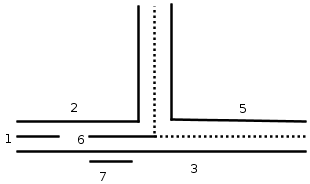
\includegraphics[width=5cm]{./img/noClawHorizontal.png}
 \caption{Example of Construction 3 }
\label{fig:noClawHorizontal}
\end{figure}  
 

%--------------------------start F10-8OPC
\begin{lema}\label{lem:F10-8opcIsNotB1EPG}
Let $F_{10}(8)'$ be the graph with same set of vertices of $F_{8}$, see Figure~\ref{fig:16proibidos}(h), and same set of edges except by $e_1=(4,6)$ or   $e_2=(8,6)$  that may or may not belong to $E(F_{10}(8)')$. The graph $F_{10}(8)'$  $\notin B_1$-EPG. 
\end{lema}

\begin{pf}
We know that each clique in single bend representation is represented by edge-clique or claw-clique. In the graph $F_{10}(8)'$, see Figure~\ref{fig:f10-8opc}, the clique $G[2,3,6]$ belong of two maximal cliques, one with the vertex $5$ and other with the vertex $7$. So by Lemma~\ref{lem:cliquesMaximais}, the clique $G[2,3,6]$ is not represented by claw-clique. Then the paths $P_{2}$, $P_{3}$ and $P_{6}$ form  an edge-clique.

Notice that the subgraph formed by $G[1,2,3,5,7]$ plus vertex $4$ or $8$ induce a graph similar to Figure~\ref{fig:obstrucaoCentro}. So we know that if the cliques induced by $G[2,3,5]$ or $G[2,3,7]$ are represented by an edge-clique $C_e$ then satellites, relative to $C_e$, are on the same side of the clique, see Lemma~\ref{lem:obstrucaoCentro}. Further, at least one among cliques $G[2,3,1]$, $G[2,3,5]$ and $G[2,3,7]$  is represented by edge-clique because vertices $1,5$ and $7$ form an independent set adjacent to clique $G[2, 3]$. So, we can state that at least one clique among $G[2,3,1]$, $G[2,3,5]$ and $G[2,3,7]$ is represented by edge-clique and will be located with one satellite at right and another at left. Well, we know that this edge-clique can not be $G[2,3,5]$ or $G[2,3,7]$, otherwise we would have a condition like in the Lemma~\ref{lem:obstrucaoCentro}. So, the central edge-clique is $G[2,3,1]$ and satellites $5$ and $7$ are in different sides. This configuration has a problem, the vertex $6$ is adjacent to $2, 3, 5$ and $7$ then path $P_6$ must to intersect only paths $P_2, P_3, P_5$ and $P_7$. Besides $G[2,3,6]$ has to be edge-clique, the path $P_6$  should not intersect $P_1$ but it has to intersect $P_5$ and $P_7$, absurd to any $B_1$-EPG representation.  Even if there were edges $e_1$ or $e_2$ in $F_{10}(8)'$, the interval of edge-clique $G[2,3,1]$ remains as an impediment to any $B_1$-EPG representation of $F_{10}(8)'$.

Therefore, we conclude that the graph $F_{10}(8)'$ is not a $B_1$-EPG graph.
 $\square$\end{pf} 

 \begin{figure}[htb]	
 \center%6.3
 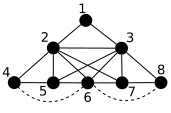
\includegraphics[width=4cm]{./img/f10-8opc.png}
 \caption{Graph $F_{10}(8)'$ plus two optional edges.}
\label{fig:f10-8opc}
\end{figure}  
 


%------------------------- end F10-8OPC
\begin{coro}\label{coro:f8}
Let $G$ be the graph $F_{8}$, see Figure~\ref{fig:16proibidos}(h). $G \notin B_1$-EPG. 
\end{coro}
\begin{pf}
The proof is immediate by Lemma~\ref{lem:F10-8opcIsNotB1EPG}. $\square$
\end{pf}

\begin{coro}\label{coro:f9}
Let $G$ be the graph $F_{9}$, see Figure~\ref{fig:16proibidos}(i). $G \notin B_1$-EPG. 
\end{coro}
\begin{pf}
The proof is immediate by Lemma~\ref{lem:F10-8opcIsNotB1EPG}. $\square$
\end{pf}



\begin{coro}\label{coro:F108IsNotB1EPG}
Let $G$ be the graph $F_{10}(8)$, see Figure~\ref{fig:ktent}. $G \notin B_1$-EPG. 
\end{coro}

\begin{pf}
The proof is immediate by Lemma~\ref{lem:F10-8opcIsNotB1EPG}. $\square$
\end{pf}

% \begin{pf}
% The graph $F_{10}(8)$, also known as $k$-tent, is a minimal forbidden subgraph to interval graphs, see~\cite{lekkeikerker1962representation}. Thus $F_{10}(8)$ is not an interval graph, so some path in an EPG representation of $F_{10}(8)$ has at least one bend.

% We know that each clique in single bend representation is represented by edge-clique or claw-clique. The graph $F_{10}(8)$ has 2 graphs $K_{4}$ as subgraphs, and these $K_{4}$\textsc{\char13}s share 3 vertices. Suppose that one of these cliques is represented by claw-clique with center in $(x_0, y_0)$, e.g. $G[2,3,5,6]$. As $P_{2}$, $P_{3}$ and $P_{6}$ belong of two maximal cliques, one with path $P_{5}$ and other with path $P_{7}$ then by Lemma~\ref{lem:cliquesMaximais} the paths $P_{2}$, $P_{3}$ and $P_{6}$ are not represented by claw-clique. Then the paths $P_{2}$, $P_{3}$ and $P_{6}$ are always represented by a edge-clique.

% Notice that the subgraph formed by $G[1,2,3,5,7]$ plus vertex $4$ or $8$ forms graph similar to Figure~\ref{fig:obstrucaoCentro}. So we know that if the cliques induced by $G[2,3,5]$ or $G[2,3,7]$ are represented by an edge-clique $C_e$ then satellites, relative to $C_e$, are on the same side of the clique, see Lemma~\ref{lem:obstrucaoCentro}. Further, at least one among cliques $G[2,3,1]$, $G[2,3,5]$ and $G[2,3,7]$  is represented by edge-clique because vertices $1,3$ and $5$ form an independent set adjacent to clique $G[2, 3]$. So, we can state that at least one clique among $G[2,3,1]$, $G[2,3,5]$ and $G[2,3,7]$ is represented by edge-clique and will be located with one satellite at right and another at left. Well, we know that this edge-clique can not be $G[2,3,5]$ or $G[2,3,7]$, otherwise we would have a condition like in the Lemma~\ref{lem:obstrucaoCentro}. So, the central edge-clique is $G[2,3,1]$ and satellites $5$ and $7$ are in different sides. This configuration has a problem, the vertex $6$ is adjacent to $2, 3, 5$ and $7$ then path $P_6$ must to intersect only paths $P_2, P_3, P_5$ and $P_7$. Besides $G[2,3,6]$ has to be edge-clique, the path $P_6$ does not intersect $P_1$ but it has to intersect $P_5$ and $P_7$, absurd to any $B_1$-EPG representation.  

% Therefore, we conclude that the graph $F_{10}(8)$ is not a $B_1$-EPG graph.
%  $\square$\end{pf} 

 \begin{figure}[htb]	
 \center%6.3
 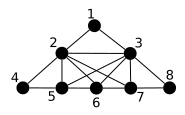
\includegraphics[width=4.5cm]{./img/ktent.png}
 \caption{Graph $F_{10}(8)$.}
\label{fig:ktent}
\end{figure}  
 


\begin{lema}\label{lem:f10}
The graph $F_{10}(n)$ $\notin B_1$-EPG. 
\end{lema}

\begin{pf}
The graph $F_{10}(n)$ presented in~\cite{alcon2015characterizing}, see Figure~\ref{fig:16proibidos}(j), is a graph that has $n$ vertices and whose set $K$ is highlighted. This graph has $k=n-5$ vertices, where $k\geq 3, n\geq 8$. Note that each clique $\{a, b, i\}$, where $i \in K$ and  $2\leq i \leq k-1$, have same  characteristic of the clique $\{2, 3, 6\}$  of graph $F_{10}(8)$ presented in Figure~\ref{fig:ktent}, i.e. in any single bend representation these set of vertices are represented by edge-clique.

We will prove that there exists a single bend representation for $F_{10}(n)$ if only if there exists a single bend representation for $F_{10}(n-1)$. Our induction  is about the set of vertices of $K$ and the paths that represent them.

% \begin{figure}[htb]	
 \center%6.3
 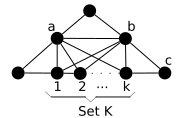
\includegraphics[width=4cm]{./img/f10n.png}
 \caption{Graph $F_{10}(n)$}
\label{fig:f10n}
\end{figure}  
 


Given a graph $F_{10}(n)$, suppose there is a $B_1$-EPG representation $R$ for $F_{10}(n)$. By Lemma~\ref{lem:cliquesMaximais} each clique $\{a, b, i\}$, where $i \in K$ and  $2\leq i \leq k-1$ is an edge-clique, then we need analyze two cases:

\begin{itemize}
    \item case 1: Paths $\displaystyle P_{{k-1}}$ and $\displaystyle P_{{k}}$ are on same row/column.
    
    The interval between row/column where $ P_{{1}}$ intersects $ P_{{2}}$ through row/column that $ P_{{k-1}}$ intersects $ P_{{k}}$  necessarily has only paths of set $P_i \cup \{P_a,P_b\}$. No path $P_i$, $2 \leq i \leq k-1$, needs bend, except if $P_a$ or $P_b$ bend.
     As $R$ is a valid single bend representation for $F_{10}(n)$ then when we remove the path $\displaystyle P_{{k}}$, we can preserve the intersection of $P_{{k}}$ in $P_{{k-1}}$ and now we have a representation $R'$ that is also a  single bend representation for $F_{10}(n-1)$.
    
      \item case 2: Paths $\displaystyle P_{{k-1}}$ and $\displaystyle P_{{k}}$ are on distinct rows/columns.
      
      Path $\displaystyle P_{{k}}$ is intersecting to $P_a, P_b, P_c$ and $\displaystyle P_{{k-1}}$. Path $P_c$ intersects $P_b$ and $\displaystyle P_{{k}}$. If $\displaystyle P_{b}$ bends then $P_b \cap P_c$ has that occur on this row/column. Or $\displaystyle P_{{k}}$ or $\displaystyle P_{{k-1}}$ has bend, and when we remove $\displaystyle P_{{k}}$ then $\displaystyle P_{{k-1}}$ has bend and now there exists $P_b \cap  P_c \cap $ $\displaystyle P_{{k-1}}$. If before removal $\displaystyle P_{{k}}$ the representation $R$ was a single bend representation for $F_{10}(n)$ then now $R'$ remains a single bend representation, but for $F_{10}(n-1)$.    
\end{itemize}

Yet by induction we know that there is a single bend representation for $F_{10}(9)$ if only if there is a single bend representation for $F_{10}(8)$, but by Corollary~\ref{coro:F108IsNotB1EPG} the graph $F_{10}(8)$ is not $B_1$-EPG, therefore we can conclude that $F_{10}(n) \notin B_1$-EPG.
%Thus $F_{10}$ is not a interval graph, so some path in an EPG representation of $F_{10}$ has at least one bend.
 $\square$\end{pf} 


% \begin{figure}[htb]	
 \center%6.3
 \includegraphics[width=4cm]{./img/f8.png}
 \caption{Graph $F_{8}$}
\label{fig:f8}
\end{figure}  
 

% \begin{lema}\label{lem:f8}
% The graph $F_{8} \notin B_1$-EPG. 
% \end{lema}

% \begin{pf}
% In the graph $F_{8}$, see Figure~\ref{fig:f8}, the following cliques have be represented by edge-clique in any single bend representation: $ G[2,3,6], G[3,6,7], G[2,5,6]$ , see Lemma~\ref{lem:cliquesMaximais}.

% Notice that the induced subgraph formed by $G[1,2,3,5,7]$ plus vertex $4$ or $8$ forms graph similar to Figure~\ref{fig:obstrucaoCentro}. So we know that if the cliques induced by $G[2,3,5]$ or $G[2,3,7]$ are represented by an edge-clique $C_e$ then satellites, relative to $C_e$, are on the same side of the clique, see Lemma~\ref{lem:obstrucaoCentro}. Further, at least one among cliques $G[2,3,1]$, $G[2,3,5]$ and $G[2,3,7]$  is represented by edge-clique because vertices $1,3$ and $5$ form an independent set adjacent to clique $G[2, 3]$. So, we can state that at least one clique among $G[2,3,1]$, $G[2,3,5]$ and $G[2,3,7]$ is represented by edge-clique and will be located with one satellite at right and another at left. Well, we know that this edge-clique can not be $G[2,3,5]$ or $G[2,3,7]$, otherwise we would have a condition like in the Lemma~\ref{lem:obstrucaoCentro}. So, the central edge-clique is $G[2,3,1]$ and satellites $5$ and $7$ are in different sides. This configuration has a problem, the vertex $6$ is quasi-universal, i.e. $6$ is adjacent to all vertices except  $1$. Besides $G[2,3,6]$ has to be edge-clique, the path $P_6$ does not intersect $P_1$ but it has to intersect $P_5$ and $P_7$, absurd to any $B_1$-EPG representation.  
%  $\square$\end{pf} 


% \begin{figure}[htb]	
 \center%6.3
 \includegraphics[width=4cm]{./img/f9.png}
 \caption{Graph $F_{9}$}
\label{fig:f9}
\end{figure}  
 

% \begin{lema}\label{lem:f9}
% The graph $F_{9} \notin B_1$-EPG. 
% \end{lema}

% \begin{pf}
% In the graph $F_{9}$, see Figure~\ref{fig:f9}, the following set of vertices have be represented by edge-clique in any single bend representation: $\{ 2,3,6\}, \{3,6,7\}$ , see Lemma~\ref{lem:cliquesMaximais}. 

% Notice that the induced subgraph formed by $G[1,2,3,5,7]$ plus vertex $4$ or $8$ forms graph similar to Figure~\ref{fig:obstrucaoCentro}. So we know that if the cliques induced by $G[2,3,5]$ or $G[2,3,7]$ are represented by an edge-clique $C_e$ then satellites, relative to $C_e$, are on the same side of the clique, see Lemma~\ref{lem:obstrucaoCentro}. Further, at least one among cliques $G[2,3,1]$, $G[2,3,5]$ and $G[2,3,7]$  is represented by edge-clique because vertices $1,3$ and $5$ form an independent set adjacent to clique $G[2, 3]$. So, we can state that at least one clique among $G[2,3,1]$, $G[2,3,5]$ and $G[2,3,7]$ is represented by edge-clique and will be located with one satellite at right and another at left. Well, we know that this edge-clique can not be $G[2,3,5]$ or $G[2,3,7]$, otherwise we would have a condition like in the Lemma~\ref{lem:obstrucaoCentro}. So, the central edge-clique is $G[2,3,1]$ and satellites $5$ and $7$ are in different sides. This configuration has a problem, the vertex $6$ is quasi-universal, i.e. $6$ is adjacent to all vertices except  $1$ and $4$. Besides $G[2,3,6]$ has to be edge-clique, the path $P_6$ does not intersect $P_1$ but it has to intersect $P_5$ and $P_7$, absurd to any $B_1$-EPG representation.  

% Therefore to graph $F_{9}$ does not exist a single bend representation.
%  $\square$\end{pf} 


\begin{lema}\label{lem:f6}
The graph $F_{6} \notin B_1$-EPG. 
\end{lema}

\begin{pf}
The graph $F_6$, see Figure~\ref{fig:16proibidos}(f), has the graph $G''$ as induced subgraph and by Lemma~\ref{lem:cb''} is not a $B_1$-EPG graph. Thus $F_6$ also is not a $B_1$-EPG graph.

% \begin{figure}[htb]	
 \center%6.3
 \includegraphics[width=4cm]{./img/f6.png}
 \caption{Graph $F_6$}
\label{fig:f6}
\end{figure}  
 
 $\square$\end{pf} 

\begin{lema}\label{lem:f7}
The graph $F_{7} \notin B_1$-EPG. 
\end{lema}

\begin{pf}
The graph $F_7$, see Figure~\ref{fig:16proibidos}(g), has the graph $G''$ (generalized) as induced subgraph and by Lemma~\ref{lem:obstrucaoGeneralizada} is not a $B_1$-EPG graph. Thus $F_7$ also is not a $B_1$-EPG graph.

% \begin{figure}[htb]	
 \center%6.3
 \includegraphics[width=5cm]{./img/f7.png}
 \caption{Graph $F_7$}
\label{fig:f7}
\end{figure}  
 
 $\square$\end{pf} 



\begin{teo}\label{lem:chordalB1inVPT}
Chordal $B_1$-EPG $\subsetneq$ VPT. 
\end{teo}

\begin{pf}
By results of~\cite{Asinowski2009} we kown that when $G$ is a $B_1$-EPG graph then $G|N(i)$ is AT-free, thus $G|N(i)$ is an interval graph, but the graphs $F_{1}, F_{2}, F_{3}, F_{4}$ and $F_{5}$ have one vertex whose neighborhood is an asteroidal triple, therefore these graphs are not  $B_1$-EPG.

By Theorem 6.7 of~\cite{golumbic2009} we know that in any $B_1$-EPG representation of a graph $G$, where $C$ is a maximal clique of $G$, the branch graph $B(G|C)$ contains no chordless cycle $C_n, n\geq 4$ or chordless path $P_6$. Thus, the graphs $F_{11}, F_{12}, F_{13}, F_{14}$ and $F_{15}$ are not $B_1$-EPG.

By Corollaries~\ref{coro:f8}, \ref{coro:f9} and Lemmata~\ref{lem:f10}, \ref{lem:f6}, \ref{lem:f7} from this paper, we conclude that every minimal forbidden induced subgraphs for VPT graphs are also minimal forbidden induced subgraphs for $B_1$-EPG, so we can say that the class of Chordal $B_1$-EPG graphs is contained in the class from the VPT graphs. 
 $\square$\end{pf} 

\begin{teo}
(\cite{alcon2014recognizing}) Let $G\in$VPT and $h\geq 4$.The graph $G$ belongs to $[h,2,1]-[h-1,2,1]$ if and only if max$_{C\in\mathcal{C}(G)}(\chi (B(G|C)))=h$. The reciprocal implication is also true for $h=3$.
\end{teo}



\begin{teo}
Chordal $B_1$-EPG $\subsetneq$ EPT. 
\end{teo}

\begin{pf}
Given $G \in$ Chordal $B_1$-EPG, given $\varphi$ the set of cliques of $G$. We know that by Theorem~\ref{lem:chordalB1inVPT}, $G$ is VPT, by \cite{golumbic2009} that if $G$ is $B_1$-EPG then $\chi (B(G|C))\leq 3, \forall C \in \mathcal{C}$.

By result of~\cite{alcon2014recognizing}, we can say that $G \in [3,2,1]$, and $[3,2,1] = VPT \cap EPT$, and $[3,2,1] = [3,2,2] = EPT \cap$ Chordal  then $G \in$ Chordal EPT.
 $\square$\end{pf} 


%Demonstração EPG \in EPT

% \begin{defi}
% \textit{Edge-intersection sequences}: Let $e_i, e_j$ be edges of a representation $R$ in a $B_1$-EPG representation. We say that $P_{i,j}$ is an edge-intersection sequence if the following occurs:
% \begin{itemize}
%     \item $P_{i,j}$ is a path in the grid $Q$ and a sequence of consecutive edges in the representation $R$; and
%     \item Every edges $e_u, e_{u+1}$ of $P_{i,j}$ are:
%     \begin{itemize}
%         \item $e_u, e_{u+1} \in P_u$, and $P_u \in R$;
%         \item $e_u \in P_u$, and $e_{u+1} \in P_u \cap P_v$, and $P_u, P_v \in R$;
%         %\item $e_u, e_{u+1} \in P_u$, and $P_u \in R$;
%         \item $e_u, e_{u+1} \in P_u \cap P_v$, and $P_u, P_v \in R$; 
%         \item $e_u \in P_u \cap P_v$, and  $e_{u+1} \in P_v$, and $P_u, P_v \in R$;
%     \end{itemize}
% \end{itemize}
% \end{defi}


% \begin{lema}
% Chordal $B_1$-EPG $\subsetneq$ EPT.
% \end{lema}

% \begin{pf}
% Suppose the Lemma is false and that $G$ is a connected  Chordal $B_1$-EPG graph but not is an EPT graph. Let $R$ be a single bend representation of $G$ in a grid $Q$ such that $R \notin$ EPT. Since $R$ is an edge-intersection of paths model in single bend to $G$ and the intersection model in EPT graphs is also an edge-intersection of paths model then  there must be another characteristic of $R$ that makes it impossible for $R$ to be EPT. Suppose now that there are at least two edges $e_i, e_j$, where $e_i \in P_i$ and $e_j \in P_j$, and paths $\{P_i, P_j\} \in R$, $P_i \cap P_j = \emptyset$, such that there are two distinct edge-intersection sequences, the first one going through the edge $e_v \in P_v$, and the second going through the edge $e_w \in P_w$, where $\{P_v, P_w\} \in R$ and $P_v \neq P_w \neq P_i \neq P_j$, and both sequences of intersection pass through paths $e_i$ and $e_j$. Clearly this is a contradiction because by hypothesis $G$ is Chordal and the induced subgraph by vertices corresponding to paths $[P_i, \dots, P_v, \dots, P_j]$ and $[P_i, \dots, P_w, \dots, P_j]$ forms a cycle, a contradiction. Thus, $R$ is also a tree representation for $G$. By Euler\textsc{\char13}s formula it is possible to demonstrate that every tree is planar. So taking a planar representation of $R$, then  we have an EPT representation to $G$.
%  $\square$\end{pf} 


\section{Conclusion and Open Questions}

This paper contributes by expanding what is known about $B_1$-EPG graphs and Helly property in EPG graphs. Besides we also present a characterization for subfamilies of Chordal $B_1$-EPG graphs that are contained in classes of graphs of intersection in trees, respectively VPT and EPT. We present some larger subclasses that encompass results already mentioned in the literature, see~\cite{ries2009}, and give more general characterizations for a Helly graph subfamily, see diagram depicted in Figure~\ref{fig:diagramS3Free}. 
 
 In addition to encompassing the $\{$Bull,$C_4\}$-free graph family, this new set of constraints also contains diamond-free graphs, demonstrated by the Lemma~\ref{lem:b1DiamondFree} such as Helly. These results made it possible to identify new $B_1$-EPG subclasses that have the property of being helly, namely by example Cographs, Bipartite, Block, Cactus and Line-graph of bipartite graphs.
 
 \begin{figure}[htb]	
 \center%6.3
 \includegraphics[width=7cm]{./img/diagramS3Free.png}
 \caption{Diagram of some Helly graph classes.}
\label{fig:diagramS3Free}
\end{figure}  
 

\newcommand{\newblock}{} %corrige problemas de apresentacao \newblock em bibliographystyle
\bibliographystyle{acm}%{abbrv}%{entcs}
\bibliography{refs}


\end{document}
